\documentclass[VM.tex]{subfiles}
\tikzset{
  load/.style   = {ultra thick,-latex},
  stress/.style = {-latex},
  dim/.style    = {latex-latex},
  axis/.style   = {-latex,black!55},
}

% Drawing View
\tikzset{dimetric2/.style={
  x={(0.935cm,-0.28cm)},
  y={(0.44cm, 0.312cm)},
  z={(0.000cm, 0.943cm)},
}}
\begin{document}

\subsubsection*{Description : }
Modal analysis of a rectangular strip with axial stress ($N_2$) on short edge.
\subsubsection*{Reference : }
Arthur W.Leissa ,Vibration of Plates,NASA SP-160, pg:277, Ch:10.2. \\


\subsubsection*{Material and Geometric data : }


\begin{figure}[h!]
\centering
\subfile{NAS277_DRAW.tex}
\caption{NAS277} \label{NAS277sch}
\end{figure}
\begin{table}[ht]
\renewcommand{\arraystretch}{1.5}
\centering
\caption{Input Data}
\label{my-labelsdqf}
\begin{tabular}{|ll|ll|ll|}
\hline
\multicolumn{2}{|l|}{\cellcolor[HTML]{C0C0C0}Material Property} & \multicolumn{2}{l|}{\cellcolor[HTML]{C0C0C0}Geometric Data} & \multicolumn{2}{l|}{\cellcolor[HTML]{C0C0C0}Loading Data} \\ \hline  \hline
Young's Modulus ($E$)          & 1E11 $pa$         & Length ($a$)        & 1 $m$        & $N_2$    &  3E11 $N/m^2$      \\
Poission's Ratio ($\nu$)       & 0.3         & Breath ($b$)        & 40 $m$          &        &        \\ 
Density ($\rho$)       & 7810 $Kg/m^3$         & Thickness($t$)        & 1 $m$          &    &        \\ \hline
\end{tabular}
\end{table}




\subsubsection*{Mesh and boundary condition : }





\begin{figure}[h!]
\centering
\begin{subfigure}{0.45\textwidth}
  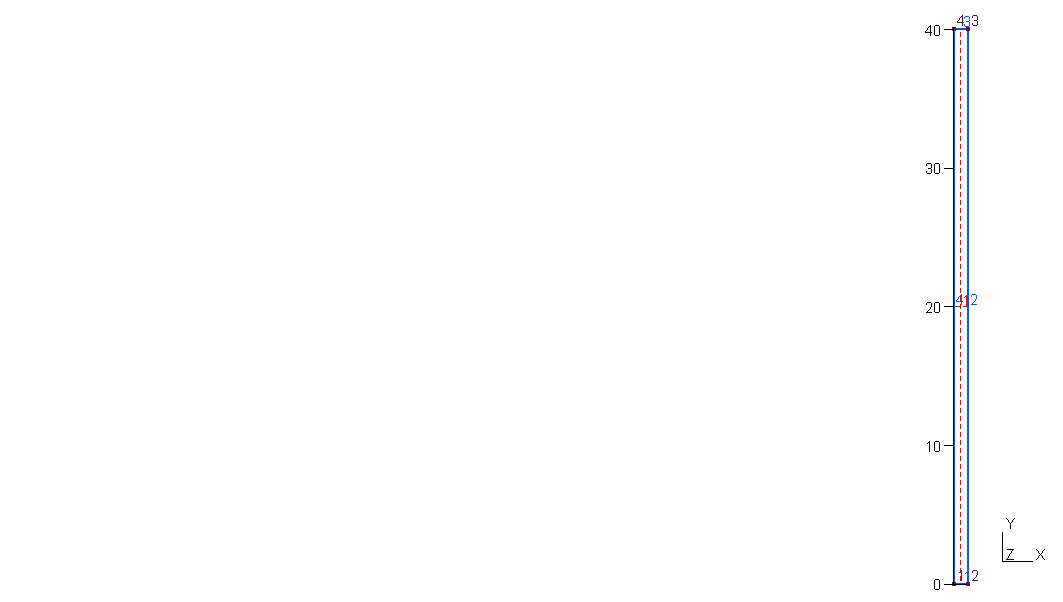
\includegraphics[width=1\linewidth,trim={30cm 0 0cm 0},clip]{NAS277/NAS277_geo.png}
  \caption{Geomentry of the problem}\label{fig:awesome_image1}
\end{subfigure} \hfill
\begin{subfigure}{0.45\textwidth}
  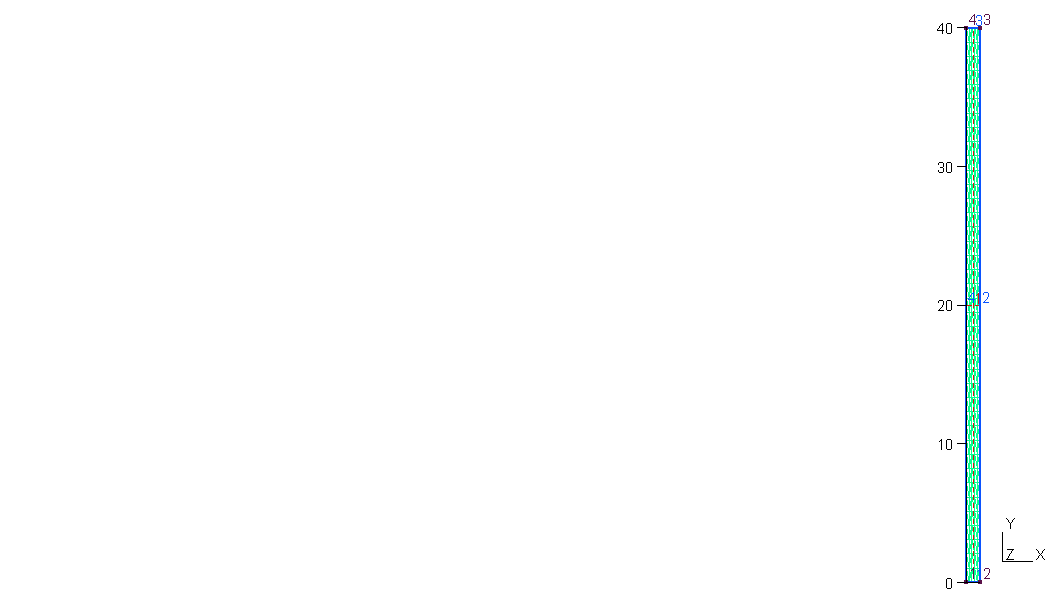
\includegraphics[width=1\linewidth,trim={30cm 0 0cm 0},clip]{NAS277/NAS277_msh.png}
  \caption{Discritization}\label{fig:awesome_image2}
\end{subfigure}
\end{figure}






\begin{table}[h!]
\renewcommand{\arraystretch}{1.5}
\centering
\caption{FEM and Boundary condition data}
\label{my-label}
\begin{tabular}{|l|lll|l|l|}
\hline
 \multicolumn{4}{l|}{\cellcolor[HTML]{C0C0C0}Direchlet Boundary} & \multicolumn{2}{l|}{\cellcolor[HTML]{C0C0C0}Loading Conditions} \\ \hline \hline
Geo - \newline Entity      & $w$          & $\theta _ x$     & $\theta _ y $    & Geo - \newline Entity         & $N_2$         \\    \hline
                 line \{1,3\}                   & Fixed      & Free         & Free        & line \{1,3\}                   & 3E11 $N/m^2$       

 \\ \hline
\end{tabular}
\end{table}
\subsubsection*{Analytically solution : }
The analytical solution of the this problem is given by 

\begin{equation}
\omega_{mn}=  \sqrt{ \frac{1}{\rho} \left( D  \left[ \left( \frac{m\pi}{a} \right)^2 + \left( \frac{n\pi}{b} \right)^2 \right] + N_1 \left( \frac{m\pi}{a} \right)^2 +N_2 \left( \frac{n\pi}{b} \right)^2 \right) }
\end{equation}

Natural frequencies are \\
mode 1 : 77.479 $Hz$ \\
mode 2 : N.A \\
mode 3 : 155.00 $Hz$ \\
mode 4 : N.A \\
mode 5 : 232.61 $Hz$ \\
mode 6 : N.A \\ \\
note : modes 2,4 and 6 are twisting modes, which are not given by the formula.
 

\subsubsection*{Result and error analysis : }


The natural frequencies of the plates are provided below.\\
mode 1 : 77.458 $Hz$ \\
mode 2 : 95.610 $Hz$ \\
mode 3 : 154.98 $Hz$ \\
mode 4 : 191.46 $Hz$ \\
mode 5 : 232.63 $Hz$ \\
mode 6 : 287.38 $Hz$ \\ 


So the Error percentage for each mode is :\\
mode 1 : 0.026 \%  \\
mode 3 : 0.012 \%\\
mode 5 : 0.013 \% \\ \\



\begin{figure}[h!]
\centering
\begin{subfigure}{.8\textwidth}
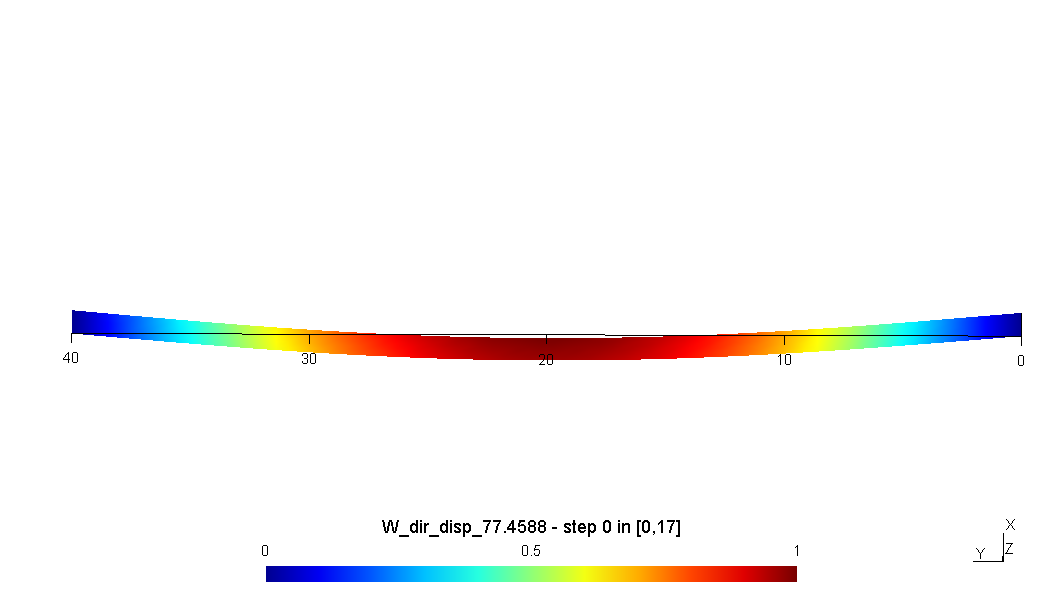
\includegraphics[width=\linewidth,trim={0 8cm 0 8cm},clip]{NAS277/NAS277_pos_1.png}
\caption{Mode Shape 1}
\end{subfigure} \vfill
\begin{subfigure}{.8\textwidth}
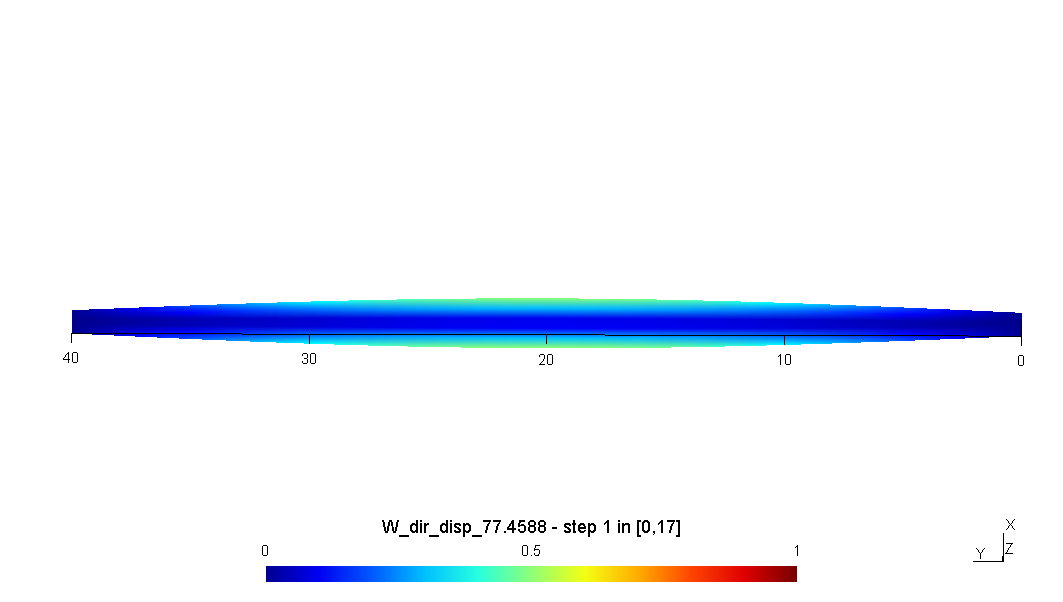
\includegraphics[width=\linewidth,trim={0 8cm 0 8cm},clip]{NAS277/NAS277_pos_2.png}
\caption{Mode Shape 2}
\end{subfigure}\vfill
\begin{subfigure}{.8\textwidth}
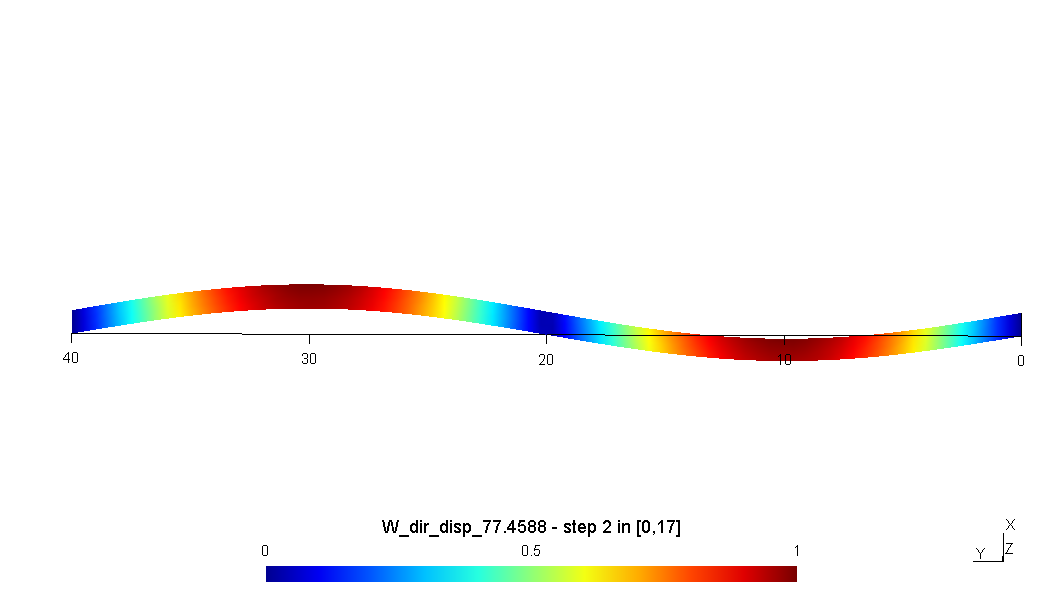
\includegraphics[width=\linewidth,trim={0 8cm 0 8cm},clip]{NAS277/NAS277_pos_3.png}
\caption{Mode Shape 3}
\end{subfigure}\vfill
\begin{subfigure}{.8\textwidth}
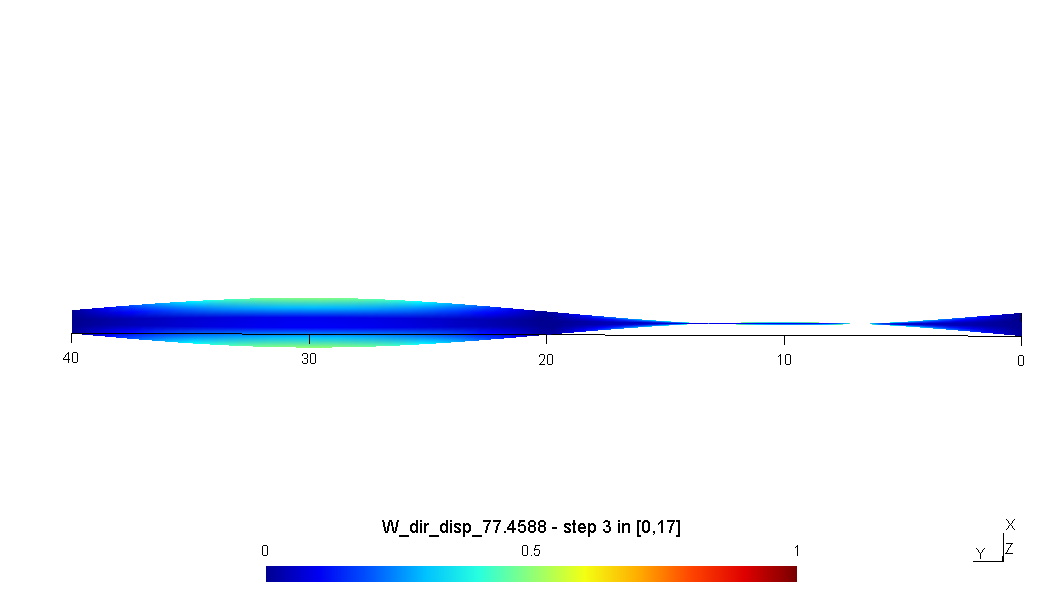
\includegraphics[width=\linewidth,trim={0 8cm 0 8cm},clip]{NAS277/NAS277_pos_4.png}
\caption{Mode Shape 4}
\end{subfigure} \vfill
\begin{subfigure}{.8\textwidth}
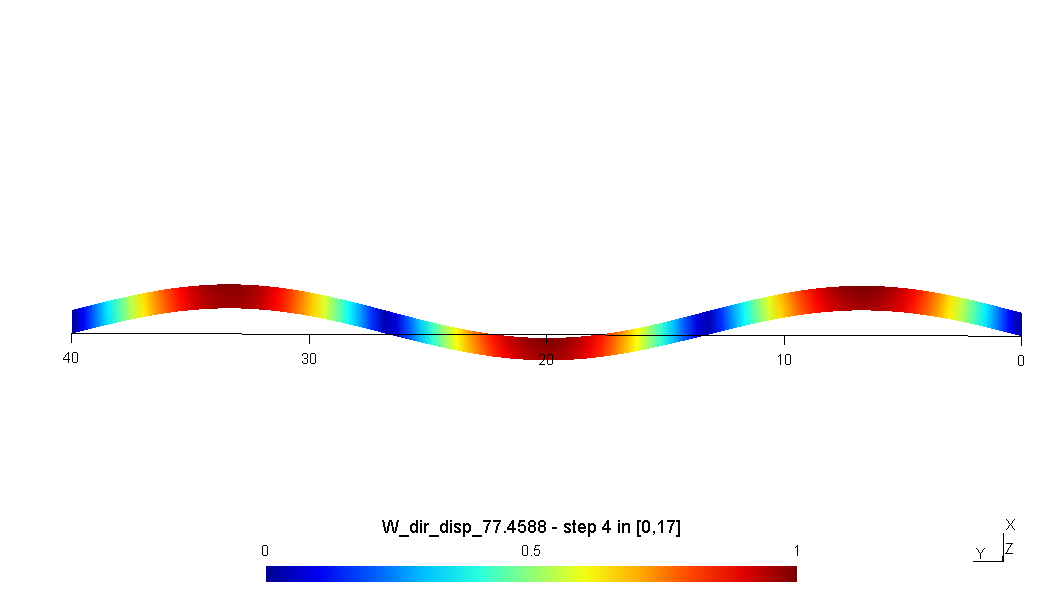
\includegraphics[width=\linewidth,trim={0 8cm 0 8cm},clip]{NAS277/NAS277_pos_5.png}
\caption{Mode Shape 5}
\end{subfigure}\vfill
\begin{subfigure}{.8\textwidth}
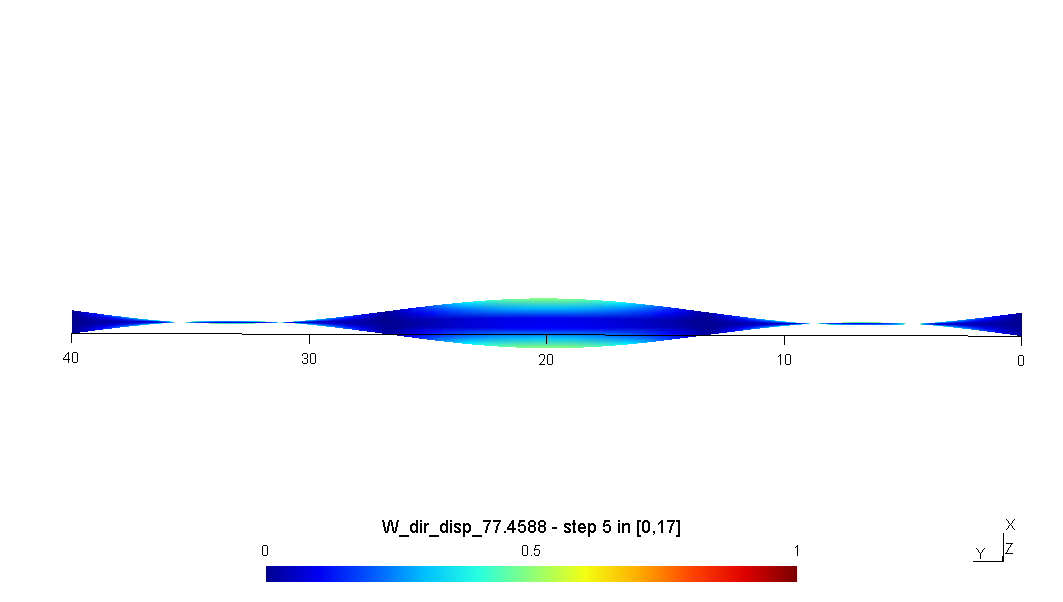
\includegraphics[width=\linewidth,trim={0 8cm 0 8cm},clip]{NAS277/NAS277_pos_6.png}
\caption{Mode Shape 6}
\end{subfigure}
\caption{Natural Modes of a rectangular strip}
\end{figure}

\end{document}